\documentclass[10pt]{article}
\usepackage{icmlko}

\icmlmeta{IP 파운데이션 월드모델}{212}{라벨을 축으로 나누면 그 축이 뒤집힌다}{웹툰의 달력 오염이 누적인지 표본인지 갈랐다. 누적이었고, 고치는 방법이 보였고, 그 방법이 축 하나를 뒤집는다}

\begin{document}

\twocolumn[
\icmlheader

\begin{abstract}
노트 211이 ``웹툰의 바닥 $-$0.969 가 누적인가 표본인가 못 가른다''를 남겼다.
갈랐다. \textbf{누적이다} --- 회차 수를 통제하면 라벨 $\leftrightarrow$
연도가 $-$0.347 에서 \textbf{$-$0.078} 로 준다(78\% 설명). 그리고
\textbf{표본이 아니다} --- 웹툰은 연재 중은 인기순, 완결은 최신순으로 뽑았는데
(노트 168), \emph{최신순}으로 뽑은 완결분 1,861건의 바닥이 $-$0.988 로
인기순 956건($-$0.810)보다 \textbf{오히려 심하다.} 표본 정렬이 원인이라면
반대여야 한다. 그럼 고치자. 회차 수로 잔차화하면 웹툰 유보 $\rho$ 가
$+$0.3895 $\to$ \textbf{$+$0.4617}, 회차당(누적 $\div$ 회차)이면
\textbf{$+$0.6853} 이다. 판도 $+$0.4654 $\to$ $+$0.4840 $\to$
\textbf{$+$0.5243} 이고 달력 몫이 $+$0.2254 $\to$ $+$0.0299 로 사라진다.
\textbf{여기서 멈춰야 한다.} 노트 207의 고침으로 \textbf{웹툰
\texttt{goods\_scale} 이 곧 회차 수다.} 라벨을 회차로 나누면 그 축이 분모가
되고, 축과 라벨의 상관이 $+$0.134 $\to$ $-$0.196(잔차) $\to$
\textbf{$-$0.741}(회차당)로 \textbf{뒤집힌다.} 축을 죽이는 정도가 아니라
반대로 세운다. 게다가 회차당은 달력도 과교정한다 --- 웹툰 달력 몫이
$+$0.350 에서 \textbf{$-$0.355} 로 넘어간다. 노트 207이 잡은 아티팩트
(분모가 작아지면 값이 터진다)의 \emph{거울상}이다. 그리고 빠진 분산을 옆
축이 흡수한다 --- \texttt{entry\_friction} 이 $+$0.301 $\to$ $+$0.391 $\to$
$+$0.502 로 세진다. \textbf{그래서 채택 안 한다.} 웹툰의 누적 오염은
실재하지만 자료 안의 재료로는 못 고친다 --- 고정 창 즐겨찾기가 필요하고
네이버 API 는 현재값만 준다. \textbf{게임은 고칠 수 있었고 웹툰은 못 한다}
--- 그 차이가 ``수집할 때 창을 같이 받았나''다.
\end{abstract}
]

\begin{figure*}[t]
\centering
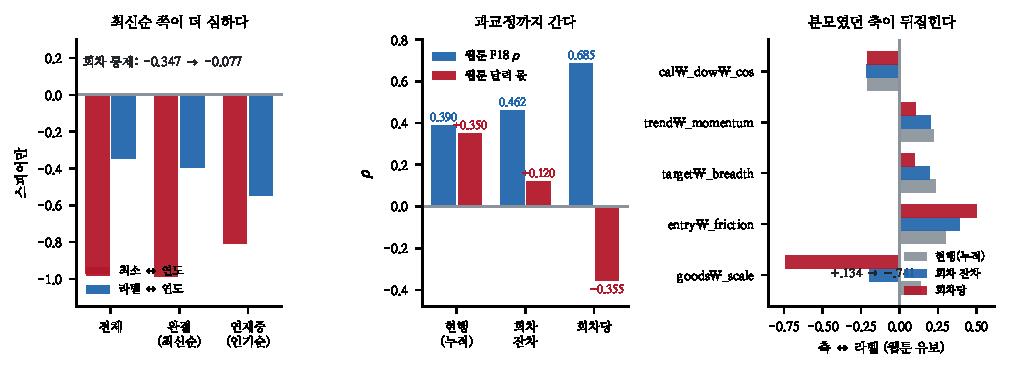
\includegraphics[width=\textwidth]{figs/selfdiv.pdf}
\caption{왼쪽 --- 최신순 쪽이 더 심하다. 가운데 --- 과교정까지 간다.
오른쪽 --- 분모였던 축이 뒤집힌다.}
\end{figure*}

\section{누적이지 표본이 아니다}

\begin{table}[t]
\centering\tsize
\caption{웹툰 2,817건을 표본 방식으로 가른다.}
\begin{tabular}{lrrr}
\toprule
& n & 라벨$\leftrightarrow$연도 & 최소$\leftrightarrow$연도 \\
\midrule
전체 & 2{,}817 & $-$.347 & $-$.973 \\
\textbf{완결(최신순)} & 1{,}861 & $-$.394 & \textbf{$-$.988} \\
연재중(인기순) & 956 & $-$.549 & $-$.810 \\
\midrule
\multicolumn{2}{l}{회차 수 통제} & \multicolumn{2}{r}{$-$.347 $\to$ \textbf{$-$.078}} \\
\bottomrule
\end{tabular}
\end{table}

\claimx{\textbf{최신순으로 뽑은 쪽이 더 심하다}($-$0.988 대 $-$0.810).
표본 정렬이 원인이라면 반대여야 한다 --- \textbf{내 예측이 반대로
틀렸다.}}{그리고 회차 수를 통제하면 78\%가 사라진다. \textbf{웹툰의 달력
효과는 누적이고, 노트 211이 도서와 같이 묶은 것이 부정확했다.}}

\section{고치면 크게 오른다}

\begin{table}[t]
\centering\tsize
\caption{라벨을 바꾸면.}
\begin{tabular}{lrrr}
\toprule
& 웹툰 $\rho$ & 웹툰 달력 & 판 F18 \\
\midrule
현행(누적) & .3895 & $+$.350 & .4654 \\
회차 잔차 & \textbf{.4617} & $+$.121 & .4840 \\
\textbf{회차당} & \textbf{.6853} & \textbf{$-$.355} & \textbf{.5243} \\
\bottomrule
\end{tabular}
\end{table}

\claimx{\textbf{웹툰 $\rho$ 가 $+$0.39 에서 $+$0.69 로 오르고 판 달력 몫이
$+$0.2254 에서 $+$0.0299 로 사라진다.} 게임에서 본 것과 같은 모양이라
채택하고 싶어진다.}{\textbf{그런데 게임은 \emph{다른} 측정(30일 창)으로
바꾼 것이고 여기는 \emph{같은} 측정을 축으로 나눈 것이다.} 그 차이가
다음 절이다.}

\section{그 축이 뒤집힌다}

\begin{table}[t]
\centering\tsize
\caption{웹툰 유보에서 축 $\leftrightarrow$ 라벨.}
\begin{tabular}{lrrr}
\toprule
& 현행 & 회차 잔차 & 회차당 \\
\midrule
\textbf{goods\_scale} & \textbf{$+$.134} & \textbf{$-$.196} & \textbf{$-$.741} \\
entry\_friction & $+$.301 & $+$.391 & \textbf{$+$.502} \\
target\_breadth & $+$.235 & $+$.194 & $+$.097 \\
trend\_momentum & $+$.220 & $+$.199 & $+$.103 \\
\bottomrule
\end{tabular}
\end{table}

\claimx{\textbf{노트 207의 고침으로 웹툰 \texttt{goods\_scale} 이 곧 회차
수다.} 라벨을 회차로 나누면 그 축이 분모가 되고 상관이 $+$0.134 에서
$-$0.741 로 뒤집힌다 --- \textbf{죽이는 정도가 아니라 반대로 세운다.}}{그리고
빠진 분산을 옆 축이 흡수한다 --- \texttt{entry\_friction} 이 $+$0.301 에서
$+$0.502 로 세진다. \textbf{웹툰 $\rho$ 가 오른 것의 상당 부분이 그
이동이다.}}

\claimx{\textbf{회차당은 달력도 과교정한다} --- 웹툰 달력 몫이 $+$0.350 에서
$-$0.355 로 넘어간다.}{노트 207이 잡은 아티팩트의 \emph{거울상}이다.
거기서는 분모(경과 주)가 최근에 작아져 값이 터졌고, 여기서는 분모(회차 수)가
최근에 작아져 값이 터진다. \textbf{같은 병을 반대 방향으로 앓는다.}}

\section{게임과 웹툰의 차이}

\claimx{\textbf{게임은 고칠 수 있었고 웹툰은 못 한다.} 게임은
\texttt{y\_w30} 이라는 \emph{다른 측정}이 레코드에 있었고, 웹툰은 같은
측정을 자기 축으로 나누는 수밖에 없다.}{그 차이가 ``수집할 때 창을 같이
받았나''다. \textbf{수집 시점에 창을 안 받으면 나중에 못 만든다} ---
네이버 API 는 현재 즐겨찾기만 준다.}

\claimx{\textbf{규약으로 적는다: 라벨을 축으로 잔차화하지 말 것.} 그 축이
뒤집히고 옆 축이 그 분산을 가져간다 --- 판이 올라도 무엇이 오른 건지
모른다.}{노트 175 · 181 · 188 · 201 이 ``이미 쓰고 있는 것을 명시로 세우면
잉여''를 네 번 봤는데, \textbf{이건 그 반대다} --- 이미 쓰고 있는 것을
라벨에서 빼면 그 축이 해로워진다.}

\begin{table}[t]
\centering\tsize
\caption{달력 오염의 세 갈래.}
\begin{tabular}{lll}
\toprule
& 원인 & 고침 \\
\midrule
\textbf{게임} & 누적 라벨 & \textbf{○} 30일 창 (노트 210) \\
\textbf{웹툰} & 누적 라벨 & \textbf{×} 창이 없다 \\
\textbf{도서} & 인기순 표본 & \textbf{×} 수집 틀 \\
펀딩 & --- & 마감 시점이라 없음 \\
\bottomrule
\end{tabular}
\end{table}

\begin{table}[t]
\centering\tsize
\caption{남은 것.}
\begin{tabular}{ll}
\toprule
\textbf{수집 규약} & 새 도메인은 창을 같이 받을 것 \\
웹툰 & 달력 몫 $+$0.350 을 안고 간다 \\
축 겹침 & 라벨과 축이 같은 재료를 쓰는 자리가 또 있나 \\
\bottomrule
\end{tabular}
\end{table}

마지막 줄이 곧바로 잴 수 있고 이 노트를 일반화한다. 웹툰에서 축
(\texttt{goods\_scale} $=$ 회차 수)과 라벨(즐겨찾기)이 같은 누적 시계를
공유하는 것을 봤다. \textbf{다른 도메인에도 축과 라벨이 같은 재료에서
나오는 자리가 있을 수 있다} --- 예컨대 세계애니의
\texttt{goods\_scale}(총 화수 $\times$ 러닝타임)과 라벨(누적 인기도),
모바일의 \texttt{goods\_scale}(앱 용량)과 라벨(누적 평점 수). \textbf{축과
라벨의 상관이 아니라 \emph{둘 다 시간과} 얼마나 붙는지를 보면 그런 자리를
찾을 수 있고}, 찾으면 그 축의 이득이 진짜인지 시계인지 갈라야 한다.

\end{document}
